\documentclass{acm_proc_article-sp}
\RequirePackage[T1]{fontenc}
\usepackage[cp1250]{inputenc}



\usepackage{pgf}
\usepackage{tikz}
\usepackage{listings}
\numberofauthors{3}
\author{
\alignauthor
J�drzej Fulara\\
\affaddr{Institute of Informatics}\\
\affaddr{University of Warsaw}\\
\affaddr{ul. Banacha 2}\\
\affaddr{02-097 Warsaw, Poland}\\
\email{fulara@mimuw.edu.pl}
\alignauthor
Krzysztof Jakubczyk\\
\affaddr{Institute of Informatics}\\
\affaddr{University of Warsaw}\\
\affaddr{ul. Banacha 2}\\
\affaddr{02-097 Warsaw, Poland}\\
\email{kjk@mimuw.edu.pl}
\alignauthor
Aleksy Schubert\\
\affaddr{Institute of Informatics}\\
\affaddr{University of Warsaw}\\
\affaddr{ul. Banacha 2}\\
\affaddr{02-097 Warsaw, Poland}\\
\email{alx@mimuw.edu.pl}
}
\bibliographystyle{abbrv}
\title{On Compiling JML Specifications into Bytecode}
\begin{document}
\maketitle


%\section{What should be in paper}
%\begin{itemize}
%	\item What is JML
%	\item What is BML
%	\item Why is translation needed??
% \item Why the tool needed?? (JVM -> VM) BML can be used to different languages, JML to one??
%	\item The tool isn't built on any existing comipler.
%	\item As input we get source file with JML annotations and compiled class file.
%	\item Therefore we can't used optimised bytecode (problem with loops, assertions etc.)
%	\item Optimized bytecode may be used for more general annotations eg. method invariants.
%	\item Detecting loops in bytecode
%	\item Description of matching source code with bytecode loops
%	\item Non-trivial example
%\end{itemize}
\maketitle
\begin{abstract}
An idea of compiling different languages to the Java bytecode becomes more and more popular. This forces us to build one common verification platform for the bytecode level. BML (Bytecode Modelling Language), a recent specification language based on JML (Java Modelling Language), is designed to be the core of such platform. There is a need to automatically translate source code level specifications into bytecode, to be able to use them later in the verification. 

In this paper we present \textit{Jml2Bml} compiler, a tool that for a given java source file with JML annotations and corresponding class file, generates BML annotations and inserts them into the bytecode.
\end{abstract}

\category{D.2.4}{Software Engineering}{Software/Program Verification}

\terms{Reliability, Verification}

\keywords{Java, byte code, JML, BML} % NOT required for Proceedings

\section{Introduction}
Modern, high level programming languages support creating software in a modular way. Applications can be divided into smaller parts that can be developed independently. In large systems, it is a common practice to outsource some well defined subsystems to external companies. The main problem in this approach is that the pieces of software developed by different programming teams often are not fully compatible. To avoid this incopatibility and useless code that is produced, there is a need to specify precisely the desired behaviour of the components, what they require and what can we expect from them. The solution is to define formally implementation contracts that can be then automatically verified.

Specification languages are useful in descirbing the system components behaviour. They are not only helpful in dividing the problem into smaller pieces, but also focus on \textit{what} is expected from each part, without saying anything about \textit{how} should it be done. The specification languages are designed to be simple enough to be understood by programmers, so they can play role of code documentation. Using specification language for documenting code has the advantage that it is possible to automatically verify that the source code implements the documented features.

One of the key aspects of modern software is security. As the end users, we usually have to trust the software we download from the internet. When the downloaded program is open source it is believed that it will not do anything inappropriate. If we download commercial software or program that is not open source, the only argument for security is a digital signature. The signature does not assure that the software is secure. There were cases when many users were deceived by respected companies eg. rootkits were installed when audio CD was inserted. The specification language can be used to describe a required security policy. In this case the verifcation stands for ensuring that the policy holds. As stated, not only the developers are interested in checking the described code property. The end user may also want to verify if the code he is running is secure. However, applications are usually distributed only in some executable form, so the specifications have also to be translated into the lower (in our case: bytecode) level. The compiled specifications are very useful in developing the Proof-Carrying Code (PCC) infrastructure \cite{pcc}.

The other reason, why it is important to be able to translate the source code specification into lower level language specifications, is the fact that more and more languages will be compiled to the same bytecode. Java Virtual Machine can be used with languages different than Java. Few examples:
\begin{itemize}
	\item Jython - the Python Java implementation
	\item JRuby - the Ruby Java implementation
	\item Jacl - the Tcl Java implementation
	\item Rhino - the JavaScript Java implementation
	\item Scala - a programming language compiled to Java bytecode
\end{itemize}
At SugarCon 2008, Sun Microsystems President and CEO Jonathan Schwartz said "we are just going to take the 'J' off the 'JVM' and just make it a 'VM'". Therefore there will be a global trend with support of companies to use JVM with languages other than Java.
Bytecode itself has a verification algorithm \cite{verification} but the verification is done only to ensure that the loaded bytecode will not cause the crash of the JVM. The verification algorithm includes:
\begin{itemize}
	\item checking that all arguments on the operand stack are legal
	\item ensuring that all types of variables passed to methods are correct
	\item checking that all load and store operations have correct types
\end{itemize}
Unfortunately programming errors are not checked. Now, the Java language has JML with proper tools that can be used to verify programs - check their correctness or find errors. Most of them operates on source code. But it seems to be a better idea to develop one common verification platform at the bytecode level, then to create multiple, different for each language platforms working at the source code level. However it would be to difficult to add annotations to the compiled programs manually, so we have to provide tools translating source code level specification languages into one common bytecode specification language. The BML, proposed in \cite{bmlBurdy} is a good choice for the target language. There are mainly three sets of tools needed to build the common bytecode verification platform:
\begin{itemize}
	\item bytecode verification tools that use BML annotations
	\item modelling languages (such as JML for Java) for other programming languages
	\item compilers that compile programs to JVM bytecode along with annotation compilers
\end{itemize}
The \textit{Jml2Bml} compiler described in this paper is designed to be a part of this scheme.

\subsection{JML}
The Java Modelling Language (JML) is a behavioural specification language for Java modules. It allows to write specifications according to \textit{design-by-contract} principles. Data types and method behaviour can be precisely commented using JML annotations. They describe the input requirements (preconditions), what we can expect at the output (postconditions) and also some lower level properties of the code (i.e. loop invariants, loop variants etc). JML annotations are written in standard Java comments, so they do not affect the normal work of any Java compiler.

An important goal in the design of JML is that it should be easily understandable by Java programmers. It is achieved by staying as close as possible to the Java syntax and semantics. The tool support for JML is rich (see \cite{overviewOfJML} for an overview). In particular, there are tools that check JML specification at runtime \cite{runtime}, in extended static checking fashion \cite{escJava}, and allow to perform software certification \cite{krakatoa}. There are also tools that support annotation generation \cite{canapa},\cite{daikon}.
\subsection{BML}
The Bytecode Modelling Language (BML) is a specification language for the bytecode. It was proposed by Burdy et al. \cite{bmlBurdy} The design of BML directly follows the fundamental concepts of JML. It inherits most constructions and keywords from the JML syntax. As the BML is developed within the MOBIUS \cite{mobius} project and the main target of the project are Java-enabled mobile devices such as mobile phones, the current version of BML assumes some simplifications of the Java bytecode which are present in the J2ME platform -- the Java platform for mobile devices with restricted resources. 

The class files representing bytecode with BML annotations are regular Java class files, executable by all Java tools. The annotations are stored within additional attributes. The BML related attributes start with the prefix \texttt{org.bmlspecs} and according to the specification of the Java Virtual Machine they should be ignored by the Machine, since their names are not part of the original JVM specification.

Of course, following the logical structure of class files, class specifications are stored as class attributes, method specifications, as attributes of corresponding method and specifications inserted in the code are attributes of the JVM Code attribute of the given method.
\section{Annotation Language}
The structure of annotations in BML and JML is very similar. We have two main types of annotations: method annotations and data type (class and interfaces) annotations.
\subsection{Method Annotations}
The most important type of method annotations are \textit{method specifications} describing the input-output behaviour of the method. This are preconditions (\texttt{requires}), defining conditions that should be fulfilled before entering the method and postconditions (\texttt{ensures}) telling what we can expect after the method finishes. One can define also which fields are modified (clause \texttt{modifies}) and which exceptions might be thrown (clause \texttt{signal}).

The other type of method annotations are specifications elements appearing in the code, like:
\begin{itemize}
\item {Assert instructions that state some facts about fields, variables etc. that should hold at this point of program execution.}
\item {Loop specifications that describe the loop invariants (\texttt{loop\_invariant}), loop variants, like  \texttt{decreases} to prove the loop's termination or \texttt{modifies} that tells which fields or variables can be changed in this loop.}
\item{Declarations of local \texttt{ghost} variables - variables that exist only in the specification. Their values can be modified only using special \texttt{set} instructions.}
\item{\texttt{Set} instructions are similar to Java assingments, but they operate on ghost fields and variables.}
\end{itemize}
\subsection{Data Type Annotations}
Class (and interface) specifications describe the behaviour of a class as a whole (in the \texttt{static} version) or of objects of that class (\texttt{instance}). The most important type of \textit{class specifications} are class invariants. They describe the property that should hold for all objects of this class in all \textit{visible} states, i.e. after all constructors and before and after all methods. For example, having a field \texttt{Object[] list}, one can write an invariant that the list is never null and its length is 10. Class invariants can be seen as additional, implicit preconditions and postcondtitions for all methods in the class.

Other important class specifications are:
\begin{itemize}
\item {Declarations of \texttt{ghost} fields. They are similar to local ghost variables, but are visible in the whole class scope.}
\item {Model fields -- fields present only in the specifications, representing some more complicated formulas. For example one can create a model field representing the property that a collection does not contain nulls.}
\end{itemize}
More details can be found in \cite{jmlrefman} and \cite{bmlrefman}.
\section{Jml2Bml Compiler}
In our work we have designed and implemented a tool called \textit{Jml2Bml} that compiles JML specifications into BML. It takes as input a Java source file with JML annotations, the corresponding class file and outputs the class file with inserted proper BML annotations. Our compiler uses an enhanced Abstract Syntax Tree for the Java source code, taken from the \textit{OpenJml} compiler. For different types of JML clauses, there are separate translation rules defined. At each node of the AST, all translation rules are applied. If some rule succeeds to translate this node, the result is stored in to the class file, using the \textit {BMLlib} library \cite{bmllib}. This approach makes the compiler easily extensible. One can simply write new translation rule to support additional features of the JML language.

Currently the \textit{Jml2Bml} compiler focuses on subset of the JML called JML Level 0. Due to external libraries limitations not all desired features are translated, for example the \texttt{loop\_modifies} clause is not supported by the \textit{OpenJml}.

The \textit{Jml2Bml} is designed to be compatible with other bytecode level tools, such as the bytecode editor \textit{Umbra}.
\subsection{Architecture Description}
In this section we present the overview of the architecture of Jml2Bml compiler. The \textit{Jml2Bml} compiler uses \textit{OpenJml} to parse the Java source code together with the JML annotations. To insert generated BML annotations, the \textit{BMLLib} library is used. The dependencies between internal packages of \textit{Jml2Bml} and \textit{OpenJml} and \textit{BMLlib} are presented in figure \ref{packages}.

The \texttt{jml2bml.main} package provides the entry point to the application. JML annotations from given source file will be translated and inserted into corresponding \texttt{class} file. Functions to access some bytecode information are located in \texttt{jml2bml.bytecode} and helpers to \textit{BMLlib} are collected in \texttt{jml2bml.bmllib}. The \texttt{jml2bml.rules} package contains translation rules for different aspects of JML. It should be easy to add new rules in the future. Classes for traversing the Java abstract syntax tree can be found in \texttt{jml2bml.ast}. In \texttt{jml2bml.symbols} implementation of symbol table can be found. The \texttt{jml2bml.engine} package contains the core translating mechanism.
\begin{figure}[h]
\centering{
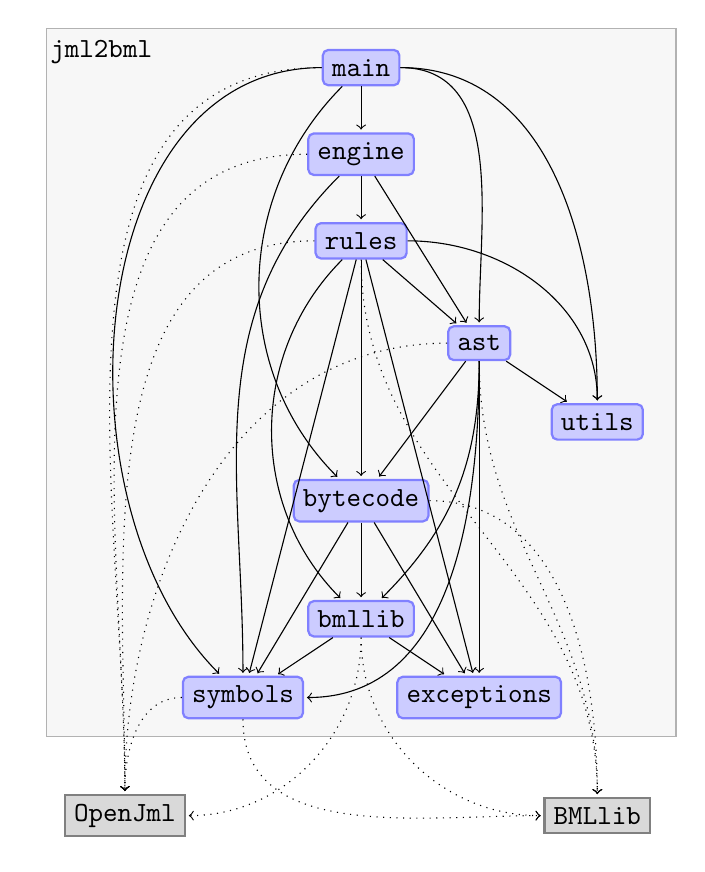
\begin{tikzpicture}[shorten >=1pt,->]
\
\tikzstyle{vertex}=[rectangle,draw=blue!50,fill=blue!20,thick,rounded corners = 2pt]
\filldraw[draw=black!30,fill=black!3] (-1,7.5) rectangle (7,-1.5);
%\draw (-0.9,7.2) node[right]{\textbf{\texttt{jml2bml}}};
\node (label) at (-0.3,7.2){\texttt{jml2bml}};
\node[vertex] (main) at (3,7) {\texttt{main}};
\node[vertex] (engine) at (3,5.9) {\texttt{engine}}  ;
\node[vertex] (rules) at (3,4.8) {\texttt{rules}}  ;
\node[vertex] (ast) at (4.5,3.5) {\texttt{ast}}  ;
\node[vertex] (utils) at (6,2.5) {\texttt{utils}};
\node[vertex] (bytecode) at (3,1.5) {\texttt{bytecode}};
\node[vertex] (bmllib) at (3, 0) {\texttt{bmllib}};
\node[vertex] (exceptions) at (4.5, -1) {\texttt{exceptions}};
\node[vertex] (symbols) at (1.5, -1) {\texttt{symbols}};
\draw (main) -- (engine);
\draw (engine) -- (rules);
\draw (rules) --(ast);
\draw (engine) -- (ast) ;
\draw(ast) -- (utils) ;
\draw(ast) -- (bytecode);
\draw (ast) to[out=270,in=45] (bmllib);
\draw (ast) -- (exceptions);
\draw (main) to[out=0,in=90] (ast);
\draw (rules) to[out=0,in=90] (utils);
\draw (rules) -- (symbols);
\draw (rules) -- (exceptions);
\draw (rules) to[out=225,in=135] (bmllib);
\draw (main) to[out=0,in=90] (utils);
\draw (main) to[out=225,in=135] (bytecode);
\draw (main) to[out=180,in=135] (symbols);
\draw (engine) to[out=225,in=90] (symbols);
\draw (ast) to[out=270,in=0] (symbols) ;
\draw (rules) -- (bytecode);
\draw (bytecode) -- (bmllib) ;
\draw (bytecode) -- (exceptions) ;
\draw (bytecode) -- (symbols) ;
\draw (bmllib) -- (exceptions) ;
\draw (bmllib) -- (symbols) ;
\tikzstyle{external}=[rectangle,draw=black!50,fill=black!15,thick]
\node[external] (BmlLib1) at  (6, -2.5) {\texttt{BMLlib}};
\node[external] (openJml) at  (0, -2.5) {\texttt{OpenJml}};
\draw[dotted] (main) to[out=180,in=90] (openJml);
\draw[dotted] (engine) to[out=180,in=90] (openJml);
\draw[dotted] (rules) to[out=180,in=90] (openJml);
\draw[dotted] (rules) to[out=270,in=90] (BmlLib1);
\draw[dotted] (ast) to[out=270,in=90] (BmlLib1);
\draw[dotted] (ast) to[out=180,in=90] (openJml);
\draw[dotted] (bytecode) to[out=0,in=90] (BmlLib1);
\draw[dotted] (bmllib) to[out=270,in=0] (openJml);
\draw[dotted] (bmllib)  to[out=270,in=180] (BmlLib1);
\draw[dotted] (symbols) to[out=180,in=90] (openJml);
\draw[dotted] (symbols) to[out=270,in=180] (BmlLib1);
\end{tikzpicture}
\caption{The dependency graph of the \textit{Jml2Bml} packages. Dotted lines denote access to external libraries.}}
\label{packages}
\end{figure}
\subsection{Translation mechanism}
The full translation contains of a set of independent translation rules. Having the set of rules the AST tree of the source code with annotations is traversed. For each visited node all translation rules are applied. For most nodes translation rules do nothing - each is responsible for few node types. The translation mechanism allows to register new rules in a very simple way, what is an important issue in case of implementing new features in the future.

\subsection{Translation rule}
The \textit{Jml2Bml} compiler uses a set of translation rules. The concept of translation rule is that it should be responsible for relatively small, independent piece of translation. For example we have separete rule for translating \textit{assert} and another one for translating \textit{loop\_invariant}. Translation rule may write results of translation to the output class file (using \textit{BMLlib}). It can hovewer only collect some translated data that may be used by other translation rules. For example both - the \textit{assert} and \textit{loop\_invariant} annotations contain expressions. Therefore we created an expression translation rule that makes translation of an expression but it does not write anything to output file - just returns the translated expression for other translation rules.

It is relatively easy to extend translation using the translation rule concept. For example if we would like to translate an annotation that was not already translated we should create a new translation rule implementation and include it in the translation mechanism by registering the rule in the translation manager. When implementing the translation rule we should first find out which AST nodes are important and then override proper methods of the base class.

Translation rule key features are:
\begin{itemize}
	\item the concept falls into a visitor design pattern
	\item translation rule is an extension of a simple abstract class
	\item translation process can be broken into smaller, independent pieces
	\item extending translation is simple
\end{itemize}

%The translation rule is a very simple but powerful concept. It uses a visitor design pattern.
%Before running the translation mechanism, translation rules need to be registered. Abstract syntax tree of the source code is traversed and for each node translation rules are executed.
%The whole tree is traversed and in each node all defined translation rules are applied. It allows also to register new rules in a very simply way, what is an important issue in case of implementing new features in the future.

\subsection{Translating expressions}
To be able to translate any JML specification, one needs to translate JML expressions, so the fundamental task in writing the compiler was to write a translation rule for expressions. As BML is based on JML, the syntax of expressions is similar in both languages and includes:
\begin{itemize}
\item{Binary arithmetic operations (+,-,*,/)}
\item{Boolean operations}
\item{Relational operators ($<$, $\le$, $\ge$, $!=$, etc)}
\item{Logical formulas containing 
\begin{itemize}
\item implications
\item quantifiers (with bound variables)
\end{itemize}     }
\end{itemize}
As in standard Java, also in JML and BML the expressions can contain local variables, references to fields (both standard and ghost), method invocations, array access etc. There can also appear constructions specific for JML and BML, like \texttt{$\backslash$old} clause. The translation of expressions is in many cases straightforward. Translation of identifiers is more complicated, because one has to distinguish between fields, ghost fields, local variables and bound variables and resolve them properly at the bytecode level.



\section{An Example of Using The\\Compiler}
This section provides an example demonstrating the result of launching the \textit{Jml2Bml}.
\subsection{Source Code}
Consider the class presented in figure \ref{source}. This is an excerpt of a class which implements a sequence of objects. We present here only one method that replaces in the \texttt{list} array the first occurence of its first parameter with the second one. True will be returned, if and only if such an element was found.

The presented code, apart from standard Java statements, contains also specifications in the JML. There is a precondition (\texttt{requires ...}) for the method \texttt{replace} defined. It requests that every time the method is invoked, the field \texttt{list} it not \texttt{null}. The next three lines (starting with \texttt{ensures} constitute the method postcondition. It states that, if the precondition was fullfiled, then the method result is true if and only if there was an element in the \texttt{list} which value has been updated from \texttt{o1} to \texttt{o2}. Note that the postcondition makes use of some JML features, like \texttt{$\backslash$result}, \texttt{$\backslash$old} or \texttt{$\backslash$exists}. This postcondition does not describe all properties of this method. For example an implementation that replaces all elements in the \texttt{list} up to the first occurence of \texttt{o1} with \texttt{o2} will fulfill this specification.

In additition to specification describing input-output behaviour of the method, also the loop implementing the \texttt{replace} method is annotated. The \texttt{loop\_invariant} clause contains the invariant: a formula that should hold at the beginning of the loop body at each loop iteration. In this example it states that in iteration \texttt{i} there are no occurences of \texttt{o1} in \texttt{list} on positions before \texttt{i}. The annotation \texttt{decreases} describes the loop variant. It specifies an expression (in this case \texttt{list.length - i}) which value is decreased in each loop iteration by at least one.


\lstset{language=java, morekeywords={requires,ensures,\result,\exists,\old,loop_invariant,\forall,==>, decreases},
        basicstyle=\small,commentstyle=\small,moredelim=*[s][\small]{/*@}{*/}}
\begin{figure}
\centering{
\begin{lstlisting}
public class List {

  private Object[] list;

  /*@ requires list != null;
    @ ensures \result ==(\exists int i;
    @ 0 <= i && i < list.length &&
    @ \old(list[i]) == o1 && list[i] == o2);
    @*/
  public boolean replace(Object o1, Object o2){
    /*@
      @ loop_invariant i <= list.length
      @ && i >=0 && (\forall int k;0 <= k
      @ && k < i ==> list[k] != o1);
      @ decreases list.length - i;
      @*/
    for (int i = 0; i < list.length; i++) {
      if (list[i] == o1) {
        list[i] = o2;
        return true;
      }
    }
    return false;
  }
}
\end{lstlisting}
}
\caption{An example class \texttt{List.java} containing single method \texttt{replace}.}
\label{source}
\end{figure}
\subsection{Bytecode}
In this section we describe the result of translating the source code from Figure \ref{source}. Since the binary class files are not human readable, we rely on its textual representation obtained from the BMLlib. The Figure \ref{bytecode} shows the translated \texttt{replace} method together with BML annotations inserted by our \emph{Jml2Bml} compiler. Lines 0 and 1 correspond to initialization the \texttt{i = 0}. The loop is located between lines 2 and 33. Lines 5 - 12 represent the \texttt{if} statement, 15 - 23 correspond to lines ??? from the source code. Loading loop condition parameters is located in lines 27 - 32 and 33 performs the loop condition comparison.

The \texttt{requires-enusers} pair is translated into input-output behaviour BML specifications located just before the method code. Loops specifications are located after line 32 in the presented listing. The Jml2Bml compiler detects loops in the bytecode and inserts the annotation before the statement representing the loop condition. In this case it is the \texttt{if\_icmplt} instruction comparing \texttt{i} and \texttt{list.length}. For more details about detecting loops refer to section \ref{loopDetection}. The modifies clause describes set of variables modified by the loop. Currently, because of \textit{OpenJML} limitations it is not supported by our compiler (the default value \texttt{everything} will be inserted).
\begin{figure}
\lstset{basicstyle=\small}

\begin{lstlisting}
/*
 * \requires true
 *  {|
 *   \precondition list != null
 *   \ensures \result ==
 *     (exists int i; 0 <= i && i < list.length
 *       && old_list[i] == o1 && list[i] == o2)
 *  |}
 */
public boolean replace(Object o1, Object o2)
0:    iconst_0
1:    istore_3
2:    goto	   #27
5:    aload_0
6:    getfield	   main.List.list
9:    iload_3
10:   aaload
11:   aload_1
12:   if_acmpne	   #24
15:   aload_0
16:   getfield	   main.List.list
19:   iload_3
20:   aload_2
21:   aastore
22:   iconst_1
23:   ireturn
24:   iinc	   %3	1
27:   iload_3
28:   aload_0
29:   getfield	   main.List.list
32:   arraylength
/*
 * \loop specification
 *   \modifies everything
 *   \invariant i <= list.length &&
 *      i >= 0 &&
 *      (forall int k; 0 <= k &&
 *          k < i==>list[k] != o1)
 *   \decreases list.length - i
 */
33:   if_icmplt	   #5
36:   iconst_0
37:   ireturn

\end{lstlisting}
\label{bytecode}
\caption{The method \texttt{replace} in the \texttt{List.class}}
\end{figure}


\section{Detecting Loops in Bytecode}\label{loopDetection}
To be able to compile the JML loop invariants, one should detect in the bytecode the corresponding loop. The created BML annotation should be associated with the bytecode instruction that represents the loop condition. Note that the loop condition is translated into multiple bytecode instructions. We are interested in the last one (comparison). A loop can be translated in one of the following ways:

\begin{figure}[h]
\centering{
\begin{tikzpicture}[shorten >=1pt,->]
\tikzstyle{vertex}=[circle,draw=blue!50,fill=blue!20,thick,minimum size=17pt,inner sep=0pt]
\foreach \name/\text/\y in {s/.../1, a/a/2, b/b/3, body/.../4, c/c/5, d/d/6, e/.../7}
\node[vertex] (G-\name) at (0,-\y) {$\text$};
\foreach \from/\to in {s/a,b/body,body/c,c/d,d/e}
\draw (G-\from) -- (G-\to);
\draw (G-a) to[out=315,in=45] (G-c);
\draw (G-d) to[out=135,in=225] (G-b);

\foreach \name/\text/\y in {s/.../1, a/a/2, b/b/3, body/.../4, c/c/5, d/d/6, e/.../7}
\node[vertex] (Q-\name) at (4,-\y) {$\text$};
\foreach \from/\to in {s/a,a/b,b/body, body/c, d/e}
\draw (Q-\from) -- (Q-\to);
\draw (Q-b) to[out=315,in=45] (Q-d);
\draw (Q-c) to[out=135,in=225](Q-a);
\end{tikzpicture}
\caption{Two ways of compiling loops.}
}
\end{figure}
In the first scenario, in the vertex \textit{a}, an unconditional jump (goto) to the vertex \textit{c} is done (vertex \textit{c} denotes loading the condition). In \textit{d} the condition is checked, and if it is fulfilled, we jump back to \textit{b}. Between \textit{b} and \textit{c} is the loop body. The annotation should be added to the vertex \textit{d}. In the second approach, the condition is tested at the beginning (\textit{a} puts the condition on the stack and \textit{b} checks it. If it is fulfilled, we enter the loop, otherwise we jump out). In \textit{c} an unconditional jump back to \textit{a} is done. The BML annotation should be associated with the instruction in the vertex \textit{a}.

\texttt{Do-while} loops and loops with always true condition (i.e. \texttt{while(true)\{...\}} or \texttt{for(;;)\{...\}} are usually compiled in another way:

\begin{figure}[h]
\centering{
\begin{tikzpicture}[shorten >=1pt,->]
\tikzstyle{vertex}=[circle,draw=blue!50,fill=blue!20,thick,minimum size=17pt,inner sep=0pt]
\foreach \name/\text/\x in {s/.../1, a/a/2, body1/.../3, b/b/4, body2/.../5, c/c/6, d/.../7}
\node[vertex] (G-\name) at (\x,0) {$\text$};
\foreach \from/\to in {s/a,a/body1, body1/b, b/body2, body2/c}
\draw (G-\from) -- (G-\to);
\draw (G-b) to[out=315,in=225] (G-d);
\draw (G-c) to[out=135,in=45] (G-a);
\end{tikzpicture}
\caption{Compiling \texttt{do-while} loop.}}
\end{figure}
Before entering the loop (between \textit{a} and \textit{c}), no condition is checked. There might be some \texttt{break} inside (vertex \textit{b}).
In this cases, the annotation should be added to \textit{a} (start of the loop). The Jml2Bml compiler covers all the cases described above. It tries to detect the first kind of loop. If it fails, tries to detect the second one. At the end checks the \texttt{do - while} case. In the first case:
\begin{itemize}
\item{assume that the tested instruction is in vertex \textit{c}. Consider all incoming edges that start in a vertex \textit{v}, which is before \textit{c}}
\item{if there are no such vertices, return null (tested instruction is not the \textit{c} vertex in the first kind loop)}
\item{else take this \textit{v} that has the longest jump to \textit{c} (other jumps come from some continue instructions inside the loop). This is \textit{a} from our graph,}
\item{look at the next instruction. This is our \textit{b}. Find the longest backward jump. It is our vertex \textit{d}}
\item{return d}
\end{itemize}
If no loop of the first kind was detected for an instruction, try to detect the second kind:
\begin{itemize}
\item{assume that the tested instruction is \textit{a}.}
\item{if the instruction has less than two incomming edges - return null}
\item{find \textit{v} that is after \textit{a} and has the longest jump to it. This is \textit{c} from our graph.}
\item{look at the next instruction \textit{d}.}
\item{find such \textit{u} that there exist an edge (\textit{u},\textit{d}) and \textit{u} is between \textit{a} and \textit{d} and there is no such \textit{u'} that \textit{u'} is between \textit{a} and \textit{u} and there is an edge (\textit{u'},\textit{d}). This is candidate for \textit{b}}
\item{if at \textit{u} is an unconditional jump (goto), then this is a break - this is the case of loop with always true condition. Return \textit{a}}
\item{else (at \textit{u} is a conditional jump) - \textit{u} is really our \textit{b}. Return it.}
\end{itemize}
If both cases described above fail, the algorithm tries to detect the \texttt{do - while} loop. We simply check if
\begin{itemize}
\item{there is a backward jump from the tested instruction to some \textit{a}}
\item{if yes, assuming that cases 1 and 2 failed, return \textit{a} as the beginning of the loop}
\end{itemize}

\section{Matching Bytecode Loops with Source Loops}
Let us take any source method that has loop with JML invariant and bytecode corresponding to this method. The compiler used to generate the bytecode may have used some optimizations. Unfortunately this causes some problems. Here are some exemplary loop optimizations:
\begin{itemize}
	\item loop unwinding (loop unrolling)\\
In this case invariant should be put in every copy of the loop. But the invariant may need a change.
	\item loop interchange\\
If internal loop invariant depended on external loop variables - this invariant must also be translated.
	\item code-motion\\
Some part of code may be moved before the loop. What if invariant depended on it?
\end{itemize}
When we want to add BML specifications to optimized bytecode, we have to know the optimizations that were used. There are two solutions of this problem:
\begin{itemize}
	\item Include the JML to BML compiler in existing Java compiler application.
	\item Use non-optimizing compiler.
\end{itemize}
The first solution has the advantage that even optimized bytecode may be annotated. Unfortunately it would have to use an existing compiler infrastructure so every change in the compiler might reflect a change in translating annotations. This would be very difficult and complicated.

In second solution translations are more predictible and simplier compared to the optimizing compiler. Different compiler implementations may be used eg. Jikes or the reference one.

In both cases class level annotations (method pre-post conditions, class invariants) can be translated in the same way. Therefore when we limit to only these annotations we can use Jml2Bml compiler even with an optimizing compiler.
\section{Related Work}
\textit{Jml2Bml} compiler uses external libraries that are still in developement (\textit{BMLlib}, \textit{OpenJML}). They do not provide whole functionality needed to compile the JML Level 0. When they get more powerful, also our compiler should be enhanced to support more sophisticated specifications (and therefore get more adequate for the end user). The most urgent are the \texttt{modifies} clauses and \texttt{set} instructions.
\section{Conclusion}
We have presented \textit{Jml2Bml} compiler that deals with JML annotations and translates them into BML. The resulting annotations are inserted in binary format into the class file (using the \textit{BMLlib} library). The compiler is an important step in building a common verification platform for all languages compiled to the Java bytecode.
\bibliography{jml2bml}
\end{document}
